\begin{question}
\noindent Triangle $T$ has vertices $A(1,1)$, $B(3,1)$ and $C(1,2)$.

\noindent Triangle $T$ is first reflected in the line $y = x$ to give triangle $T_1$.

\noindent Triangle $T_1$ is then reflected in the line $x = 0$ (the $y$-axis) to give triangle $T_2$.

\begin{center}
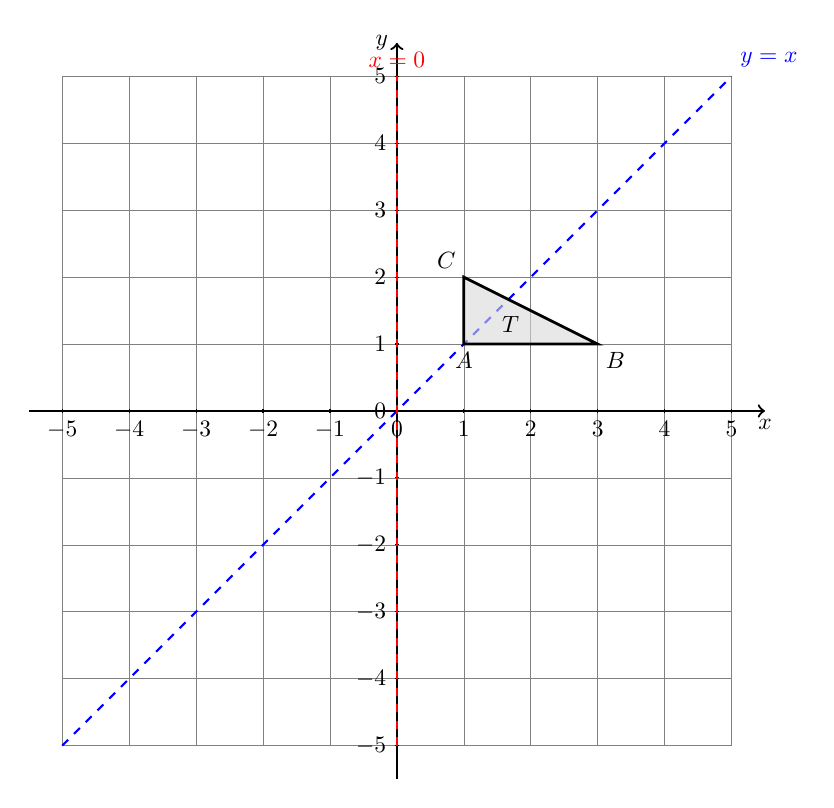
\begin{tikzpicture}[scale=0.85, transform shape]
    % Define colours
    \definecolor{borderColour}{HTML}{000000}
    \definecolor{fillColour}{HTML}{D8D8D8}

    % Define axis scale
    \def\axisLimit{5}

    % Draw grid
    \draw[step=1cm,gray,very thin] (-\axisLimit,-\axisLimit) grid (\axisLimit,\axisLimit);

    % Draw axes
    \draw[thick,->] (-\axisLimit-0.5,0) -- (\axisLimit+0.5,0) node[anchor=north] {$x$};
    \draw[thick,->] (0,-\axisLimit-0.5) -- (0,\axisLimit+0.5) node[anchor=east] {$y$};

    % Label x-axis and y-axis
    \foreach \x in {-\axisLimit,...,\axisLimit}
        \draw (\x cm,1pt) -- (\x cm,-1pt) node[anchor=north] {$\x$};
    \foreach \y in {-\axisLimit,...,\axisLimit}
        \draw (1pt,\y cm) -- (-1pt,\y cm) node[anchor=east] {$\y$};

    % Draw mirror lines
    \draw[dashed, thick, blue] (-\axisLimit,-\axisLimit) -- (\axisLimit,\axisLimit) node[above right] {$y=x$};
    \draw[dashed, thick, red] (0,-\axisLimit) -- (0,\axisLimit) node[above] {$x=0$};

    % Define coordinates for triangle T
    \coordinate (A) at (1,1);
    \coordinate (B) at (3,1);
    \coordinate (C) at (1,2);

    % Draw triangle T
    \filldraw[fill=fillColour, draw=borderColour, line width=1pt, fill opacity=0.6] (A) -- (B) -- (C) -- cycle;

    % Label the vertices of triangle T
    \node[below] at (A) {$A$};
    \node[below right] at (B) {$B$};
    \node[above left] at (C) {$C$};
    \node at (1.7,1.3) {$T$};

\end{tikzpicture}
\end{center}

\begin{enumerate}
    \item[(a)] On the diagram (or using coordinates), find the coordinates of the vertices of triangle $T_2$.
    \vspace{4cm}
    \answerplain{2}

    \item[(b)] Find the single transformation that maps triangle $T$ directly onto triangle $T_2$.\\
    \noindent You must give full details of this transformation.
    \vspace{4cm}
    \answerlines{3}{2}
\end{enumerate}
\end{question}
